\documentclass{article}

\usepackage[english]{babel}
\usepackage[utf8]{inputenc}
\usepackage{fancyhdr}
\usepackage{amsmath}
\usepackage{amssymb}
\usepackage{setspace} 
\usepackage{graphicx}
\usepackage{float}
\usepackage{tabularx}


\pagestyle{fancy}
\fancyhf{}
\lhead{CIV102: Formula sheet}
\rhead{Youssef El Mays}
\doublespacing

\newcommand{\SubItem}[1]{
    {\setlength\itemindent{15pt} \item[-] #1}
}

\newcolumntype{L}{>{\centering\arraybackslash}m{3cm}}


\begin{document}
    \title{CIV102: Formula Sheet}

    \section{Stress, Strain}
        \begin{math} 
            \sigma = \frac{F}{A} \\
            \epsilon = \frac{\Delta l}{L} \\
            \sigma = E\epsilon  \\
            \frac{F}{A} = \frac{E \cdot \Delta l}{L}, F = \frac{AE}{L} \cdot \Delta l = k \Delta l  \\
            k = \frac{AE}{L}  \\
            W = \frac{1}{2}k\Delta x^2 
            = \frac{1}{2} F\Delta x 
            = \frac{1}{2} \sigma A \epsilon L 
            = \frac{\sigma^2 V_0}{2E} 
            = \frac{\sigma \epsilon V_0}{2}\\ 
            U = \int \sigma d\epsilon \\
            W = U \cdot V_0 \rightarrow U = \frac{W}{V_0} \\
            \epsilon_{th} = \alpha \Delta T \\
            F_{failure} = A\sigma_y \\
            F_{allowable} = \frac{A\sigma_y}{FOS} \geq F_{demand} \\
            A \geq \frac{FOS \cdot F_{demand}}{\sigma_y}
        \end{math}

    \section{Equilibrium}  
        \begin{math}
            \Sigma F = 0,\;\Sigma M = 0,\;if\;a = 0,\;where\;F = ma,\;and\;M = Fd
        \end{math}
    
    \section{Bridges}
        \begin{math}
            T_{supY}=\frac{WL}{2} \\
            T_{supX}=\frac{WL^{2}}{8h} \\
            T_{supMax}=\sqrt{(\frac{WL}{2})^{2} + (\frac{WL^{2}}{8h})^2}, \\
        \end{math}
        Given loads placed equidistantly over the span

    \section{Rotation}
        \subsection{Motion}
        \begin{math}
            I_{m} = my^{2},\;for\;a\;single\;point\;mass\\
            I_{m} = \int_{M} y^2 dm = \rho \int_A y^2 dA \\
            I = \int_A y^2 dA\\
            I = \frac{bh^3}{12}, \;for\;a\;rectangle\;(comes \;from\;integrating) \\
            F=ma=my\\
            M=F_{x}y=my^{2} \cdot \alpha = I_{m}\alpha \\
            \omega = \frac{d^{2}\theta}{dt^{2}} \\
            \theta = \omega_{i}t + \frac{1}{2}\alpha t^{2} \\   
            a = \alpha y \\
            M = Fy = m\alpha y^2 = I_m \alpha
        \end{math}
        \subsection{Bending}
        \begin{figure}[H]
            \centering
            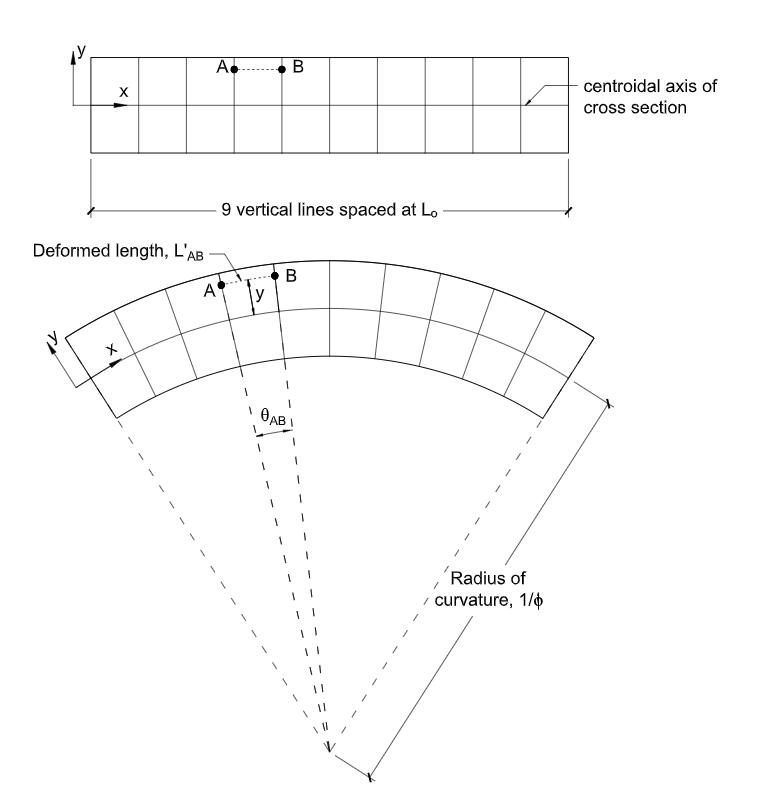
\includegraphics[width=6cm]{Bending.png}
        \end{figure}
        \begin{math}
            \phi = \frac{d\theta}{dx} \\
            L^\prime_{AB} = \phi L_0 \cdot (y +\frac{1}{\phi}) = \phi y L_0 + L_0 \\
            \epsilon(y) = \frac{\Delta l}{L_0} = \frac{L^\prime_{AB} - L_0}{L_0} = \phi y,\;\epsilon\; at\; the \; centroidal\; axis\; is\;0\\
            \sigma = E\epsilon \rightarrow \sigma(y) = E\phi y \\
            \sigma = F/A \rightarrow \Delta F = \sigma(y)\Delta A \\
            M =Fd \rightarrow \Delta M = \Delta Fy = \phi E y^2 \Delta A \\
            M = \int_A \phi E y^2 dA \\ = \phi E I
        \end{math}

    
    \section{Harmonic Motion}
        \begin{math}
            Pendulum:\;T = 2\pi \sqrt{\frac{l}{g}} \\
            Mass\;Spring:\;2\pi \sqrt{\frac{m}{k}} \\
            f = \frac{1}{T} \\
            F = -kx \\
            \omega = \frac{2\pi}{T} \\
            a = -\omega^2 x \\
            x(t) =A \cdot \sin(\omega t + \phi) \\
            v = \omega A \cdot \cos(\omega t + \phi) \\
            v = \pm \omega \sqrt{x_0^2 - x^2} \\
            \frac{d^2x(t)}{dt^2} = -A\omega^2 \sin(\omega_n t + \phi) \\
            E_k = \frac{1}{2}m\omega^2 (x_0^2 - x^2) \\
            E_t = \frac{1}{2}m\omega^2 x^2 \\
            \frac{1}{2}mv^2 = \frac{1}{2}kx^2 \rightarrow v = \sqrt{x\frac{k}{m}}
        \end{math}
\\
        \textbf{Gravity}\\
        \begin{math}
            m\frac{d^2x(t)}{dt^2} + kx(t)=mg \\
            x(t) = A \sin(\omega_nt + \phi) + \Delta_0 \\
            k = \frac{mg}{\Delta_0} \\
            f_n = \frac{1}{2\pi}\sqrt{\frac{mg}{\Delta_0}\cdot\frac{1}{m}} =\frac{1}{2\pi}\sqrt{\frac{g}{\Delta_0}}
        \end{math}

    \section{Staticaly Determined Structures}
        \begin{table}[H]
            \centering
            \begin{tabularx}{\textwidth}{| X | L | L | c |}
                \hline
                \textbf{Name} & 
                \textbf{Permited Degrees of Freedom} & 
                \textbf{Restrained Degrees of Freedom} &
                \textbf{Reactions} \\
                \hline
                Roller & 
                $\Delta(x \oplus y),\;\theta$ &
                $\Delta y = 0$ &
                $F_y$ \\
                \hline
                Pin &
                $\theta$ &
                $\Delta x = \Delta y = 0$ &
                $F_x,\;F_y$ \\
                \hline 
                Fixed End &
                N/A &
                $\Delta x = \Delta y = \Delta \theta = 0$ &
                $F_x,\;F_y,\;M_{xy}$ \\
                \hline
            \end{tabularx}
        \end{table}

    \section{Truss Brigde}
        \begin{figure}[H]
            \centering
            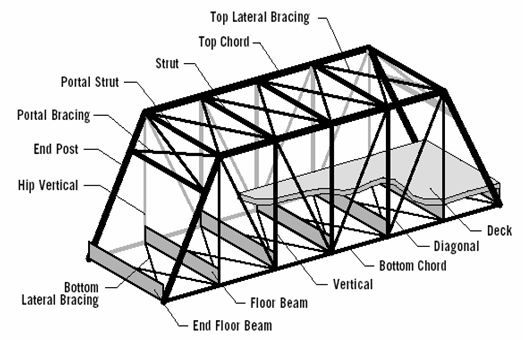
\includegraphics[width=8cm]{TrussBridge.jpeg}
        \end{figure}
        \begin{enumerate}
            \item Select Geometry
            \item Determine Loads
                \SubItem{Gravity}
                \SubItem{Wind}
            \item Analyze forces in members
            \item Design components
            \item Determine stiffeness
            \item Check dynamic forces 
            \item Iterate
        \end{enumerate}
        \begin{math}
            P_{central\;joint}= W \cdot \frac{s\cdot W_D}{2} \\
            P_{end\;joint}= W \cdot \frac{s\cdot W_D}{4} 
        \end{math}
    
    \section{Buckling}
        \begin{math}
            \phi = \frac{d\theta}{dx} \\
            P \cdot y = P \cdot \Delta_{lat} = M\\
            M = EI\phi \\
            y(x) = A \sin(\omega x + B) \\
            \frac{dy}{dx} = A\omega \cos(\omega x +B) \\
            \frac{d^2y}{dx^2} = -A\omega^2 \sin(\omega x +B) \\
            n\pi =L\cdot \sqrt{\frac{P}{EI}},\;n\;\epsilon \;\mathbb{N}\\
            P = \frac{n^2\pi^2 E I}{L^2} \\
            P_{crit} = \frac{\pi^2 EI}{L^2} = P_E \\
            r = \sqrt{\frac{I}{A}},\;r=\;radius\;of\;gyration\\
            \sigma_E = \frac{P_E }{A} = \frac{\pi^2 EI}{AL^2} = \frac{\pi^2 E}{(L/r)^2},\;L/r=\;slenderness\;ratio 
        \end{math}

    \section{Compression Member}
    \begin{math}
        failure\;envelope = \min\{\sigma_y, \sigma_E\} \\
        \sigma_{allowable} = \min\{\frac{1}{FOS_{crush}}\cdot\sigma_y, \frac{1}{FOS_{buckling}}\cdot\sigma_E\} \\
        Yield:\;F_{allowable}=\frac{1}{FOS_{crush}}A\sigma_Y \geq F_{demand} \\
        A \geq FOS_{crush} \cdot \frac{F_{demand}}{\sigma_Y}\\
        Buckling:\;F_{allowable}=\frac{1}{FOS_{buckling}}A\sigma_E \geq F_{demand} \\
        I \geq FOS_{buckling} \cdot \frac{F_{demand} L^2}{\pi^2 E}
    \end{math}
\end{document}
